%%%%%%%%%%%%%%%%%%%%%%%%%%%%%%%%%%%%%%%%%
% BMRB Validation Report
% LaTeX Template
% Version 1.0 (November 8, 2022)
%
% Author: Kumaran Baskaran
%%%%%%%%%%%%%%%%%%%%%%%%%%%%%%%%%%%%%%%%%


%\documentclass[12pt]{article}
%\usepackage[T1]{fontenc}
%\usepackage{mathptmx}

%\usepackage{titling}
%\usepackage{graphicx}
%\usepackage{longtable}
%\graphicspath{{Figures/}{./}}
%
%\pretitle{
%  \begin{center}
%  \LARGE
%  
\includegraphics{/logo}\\[\bigskipamount]
%}
%\posttitle{\end{center}}
%\title{\LARGE Chemical Shift Validation Report} % Report title
%
%\author{}
%
%\date{\today} % Date of the report
%
%
%\setlength{\droptitle}{-10em}
%
\documentclass[12pt]{article}

\makeatletter
\def\hyphenatestring#1{\xHyphen@te#1$\unskip}
\def\xHyphen@te{\@ifnextchar${\@gobble}{\sw@p{\hskip 0pt plus 1pt\xHyphen@te}}}
\def\sw@p#1#2{#2#1}
\makeatother
\usepackage{amsmath,amssymb}
\usepackage[parfill]{parskip}
\usepackage{mfirstuc}
%\usepackage{draftwatermark}
%\SetWatermarkLightness{ 0.9 }
%\SetWatermarkText{\today}
%\SetWatermarkScale{ 3 }
\usepackage[
%      dvipdfm,    %put here the correct(!) driver you are using
      colorlinks=true,    %no frame around URL
      linkcolor = blue, citecolor = blue, urlcolor = blue, % all links blue
%      urlcolor=black,    %no colors
%      menucolor=black,    %no colors
%      linkcolor=black,    %no colors
%      pagecolor=black,    %no colors
%      bookmarks=true,    %tree-like TOC
%      bookmarksopen=true,    %expanded when starting
%      hyperfootnotes=false,    %no referencing of footnotes, does not compile
%      pdfpagemode=UseOutlines    %show the bookmarks when starting the pdf viewer
]{hyperref}

\usepackage{hyperref}



\usepackage{graphicx}
\graphicspath{{Figures/}{./}}
%\usepackage[strings]{underscore}
\usepackage{subfig}
\usepackage{float}
\usepackage{amsmath}
\usepackage{color}
\usepackage{soul}
\definecolor{darkgreen}{rgb}{0.1,0.6,0.1}
\definecolor{lightred}{rgb}{1.0,0.7,0.7}
\definecolor{lightblue}{rgb}{0.7,0.7,1.0}
\sethlcolor{lightred}
\usepackage{longtable}
\usepackage{rotating}
\usepackage[table]{xcolor}
\usepackage{multirow}
\usepackage[margin=2cm]{geometry}
\usepackage[super, sort]{natbib}
\usepackage{tikz}
\usepackage{array}
\usepackage[T1]{fontenc}
% \usepackage[Q=yes]{examplep}

\bibpunct{(}{)}{;}{a}{,}{,} % required for natbib

\newcommand\VRule[1][\arrayrulewidth]{\vrule width #1}

\newcommand\blfootnote[1]{%
  \begingroup
  \renewcommand\thefootnote{}\footnote{#1}%
  \addtocounter{footnote}{-1}%
  \endgroup
}

\newcommand{\rectangle}[1]{\tikz{\filldraw[draw=#1,fill=#1] (0,0)
rectangle (1.6em,0.6em);}}

\newcolumntype{P}[1]{>{\centering\arraybackslash}p{#1}}
%\usepackage[us,12hr]{datetime}
\usepackage[en-US]{datetime2}
\usepackage{textcomp}
\usepackage{fancyhdr}
\setlength{\textheight}{23.8cm}
\setlength{\footskip}{1cm}
\lhead{Page \thepage}
\chead{BMRB validation reprot}
\rhead{7354}
\lfoot{}
\cfoot{ 
\includegraphics[width=6cm]{/logo}}
\rfoot{}
\renewcommand{\headrulewidth}{0.4pt}
\renewcommand{\footrulewidth}{0.4pt}

\title{

\includegraphics[]{/logo}
\\
Chemical Shift Validation Report
}


\date{\DTMsetstyle{en-US}\today ~ -- ~ \DTMcurrenttime ~ EST}



\begin{document}

\maketitle 
%This is a chemical shift validation report for a publicly released BMRB entry
\begin{center}
	\begin{tabular}{l c p{.8\linewidth}}
		Entry ID& : & 7354 \\
		Title& : & NMR STRUCTURE OF A PROTEIN-DNA COMPLEX OF AN ALTERED SPECIFICITY MUTANT OF THE LAC REPRESSOR THAT MIMICS THE GAL REPRESSOR
 \\
		Authors& : & R. K. Salinas; G. E. Folkers; A. M.J.J. Bonvin; D. Das; R. Boelens; R. Kaptein \\
		Deposited on& : & 2006-12-01 \\
		%Released on & : & date \\
	\end{tabular}
\end{center}
\vspace*{\fill}
The following versions of software and data  were used in the production of this report:
\begin{center}
	\begin{tabular}{l c l}
		PyNMRSTAR& : & 3.3.0 \\
		RCI& : & 1.1 \\
		ShiftChecker & : &1.2 \\
		LACS & : & VARLACSVER \\
		AVS & : & VARAVSVER\\
	\end{tabular}
\end{center}

\newpage
\pagestyle{fancy}
\renewcommand{\footrulewidth}{0pt}
\section{Summary}
The biological assembly is an oligomer with 4 chains made by 2 Entities.\\
\subsection{ Entity information}
\subsubsection{ Entity 1 }
\begin{longtable}{l l l}
Type &:& polymer\\
Polymer type &:& polydeoxyribonucleotide\\
Name &:& LAC-GAL\_OPERATOR\\
Sequence length &:& 22\\
Sequence &:& \multicolumn{1}{p{0.25\linewidth}}{\texttt{GAATTGTAAGCGCTTACAAT TC}}\\
\end{longtable}
\subsubsection{ Entity 2 }
\begin{longtable}{l l l}
Type &:& polymer\\
Polymer type &:& polypeptide(L)\\
Name &:& LAC\_HEADPIECE\_1-62\\
Sequence length &:& 62\\
Sequence &:& \multicolumn{1}{p{0.25\linewidth}}{\texttt{MKPVTLYDVAEYAGVSVATV SRVVNQASHVSAKTREKVEA AMAELNYIPNRCAQQLAGKQ SL}}\\
\end{longtable}

\subsection{ Chemical shift list information}
There  is 1 chemical shift list reproted.  The summary of the chemical shift data is given below\\
\begin{center}
\begin{longtable}{|l|l|}
\hline
Saveframe name & assigned\_chem\_shift\_list\_1\\
\hline
Saveframe ID & 1\\
\hline
\capitalisewords{ionic strength} & 20 mM\\
\hline
\capitalisewords{pH} & 6.0 pH\\
\hline
\capitalisewords{pressure} & 1.0 atm\\
\hline
\capitalisewords{temperature} & 315.0 K\\
\hline
Number of shifts & 876\\
\hline
Number of shift outliers & 3\\
\hline
Assignment completeness & 67.2\%\\
\hline
\end{longtable}

\end{center}
\section{Completeness}
Completeness information for Entity 1. It is a polydeoxyribonucleotide polymer\\
\begin{longtable}{|l|l|l|l|l|}
\hline
  & Total & $^{1}H$ & $^{13}C$ & $^{15}N$\\\hline
Sugar & 91/264 (34.5\%)& 91/154 (59.1\%)& 0/110 (0.0\%)& 0/0 (0.0\%) \\
\hline
Base & 57/213 (26.8\%)& 57/121 (47.1\%)& 0/47 (0.0\%)& 0/45 (0.0\%) \\
\hline
Overall & 148/477 (31.0\%)& 148/275 (53.8\%)& 0/157 (0.0\%)& 0/45 (0.0\%) \\
\hline
\end{longtable}
Completeness information for Entity 2. It is a polypeptide(L) polymer. 13 out of 13 methyl groups (LEU and VAL) were assigned stereospecifically.\begin{longtable}{|l|l|l|l|l|}
\hline
  & Total & $^{1}H$ & $^{13}C$ & $^{15}N$\\\hline
Backbone & 296/308 (96.1\%)& 120/124 (96.8\%)& 117/124 (94.4\%)& 59/60 (98.3\%) \\
\hline
Sidechain & 414/480 (86.2\%)& 282/321 (87.9\%)& 122/145 (84.1\%)& 11/20 (55.0\%) \\
\hline
Aromatic & 18/38 (47.4\%)& 9/19 (47.4\%)& 9/17 (52.9\%)& 0/2 (0.0\%) \\
\hline
Overall & 728/826 (88.1\%)& 411/464 (88.6\%)& 248/286 (86.7\%)& 70/82 (85.4\%) \\
\hline
\end{longtable}

\section{Statistically unusual chemical shifts}
The following table lists the statistically unusual chemical shifts. These are statistical measures, and large deviations from the mean do not necessarily imply incorrect assignments. Molecules containing paramagnetic centres or hemes are expected to give rise to anomalous chemical shifts\\\begin{longtable}{|l|l|l|l|l|l|l|}
\hline
Entity & Seq & Res & Atom & Shift (ppm) & Expected range (ppm) & Z-score\\\hline
2 & 12 & TYR & CG & 175.115 & 112.42 -- 146.96 & 13.15\\
\hline
2 & 22 & ARG & CB & 40.076 & 21.74 -- 39.52 & 5.31\\
\hline
2 & 35 & ARG & NH1 & 113.702 & 49.05 -- 99.42 & 7.84\\
\hline
\end{longtable}

\section{RCI}
RCI plot for the chemical shifts from the  save frame $assigned\_chem\_shift\_list\_1$\\ \includegraphics{rci_1}\\

\section{Order parameter}
Order parameter plot for the chemical shifts from the  save frame $assigned\_chem\_shift\_list\_1$\\ \includegraphics{s2_1}\\

\section{Simulated peak positions}
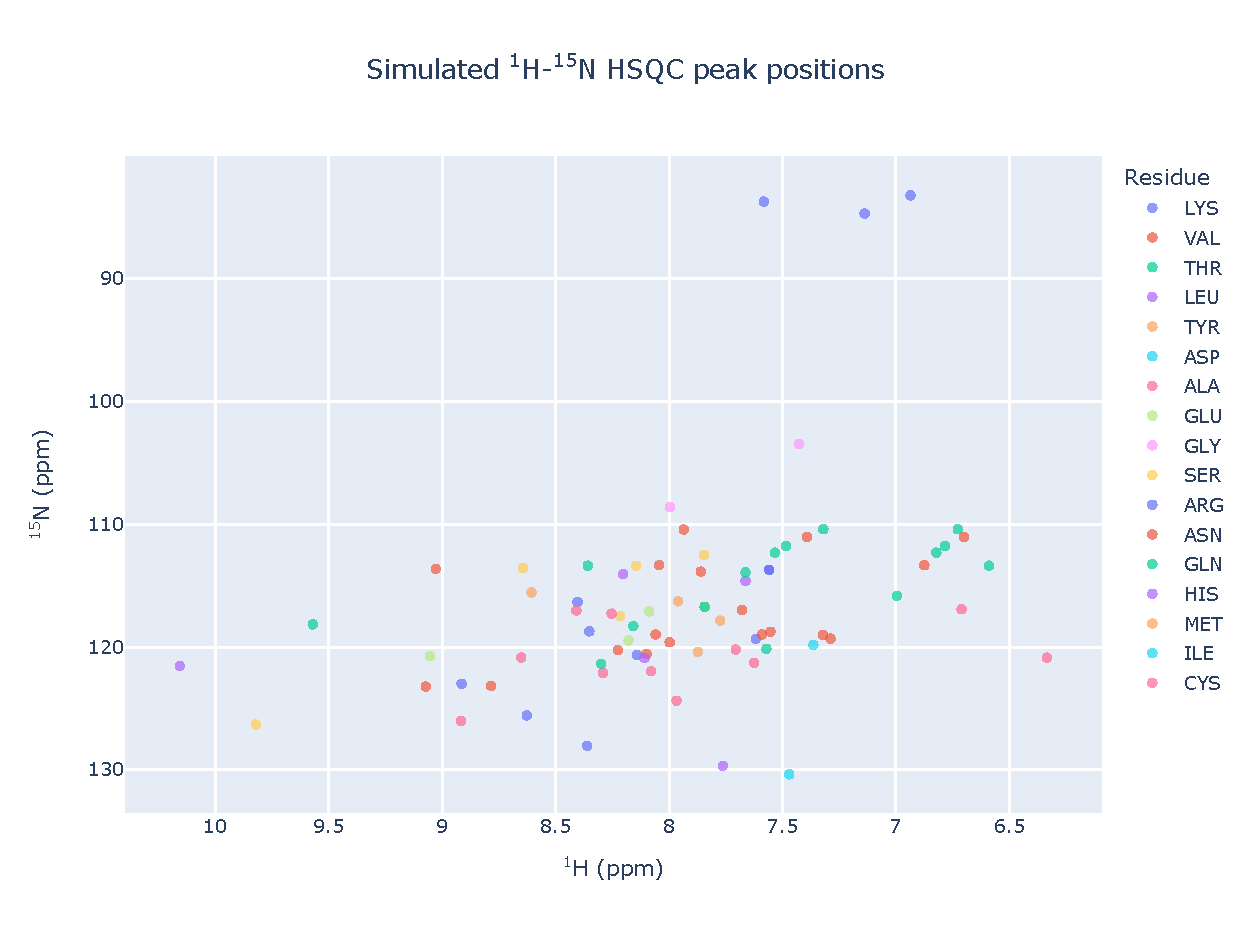
\includegraphics[width=18cm]{7354_n15.pdf}\\

\section{LACS}
Place holder for LACS results
\section{Analysis data}
place holder for the numerical values and tables.
\end{document}